
\begin{multicols*}{2}

\section{Zealot}

\lettrine[lines=3, lhang=0.15, loversize=0.25, findent=.5em]{Z}{ealots} are battle-ready warriors for whom faith is a shield, and fights for what they believe to be right. Their steadfastness gives them powers to bestow blessings to their friends and wreak cruel justice on foes.

\subsection*{Lay on Hands}

As a bonus action, you can spend one stamina point and a creature of your choice that you touch you regains Hit Points equal to 1d6 + your Spellcasting Ability modifier.

Alternatively, you can expend one stamina point to cure the target of one disease or neutralize one poison affecting it.

You can both heal and cure multiple diseases and neutralize multiple poisons with a single use of Lay on Hands, expending stamina points separately for each one.


\subsection*{Sacred Immolation}

\subsection*{Divine Smite}

\subsection*{Aura of Courage}

\begin{Figure}
\centering
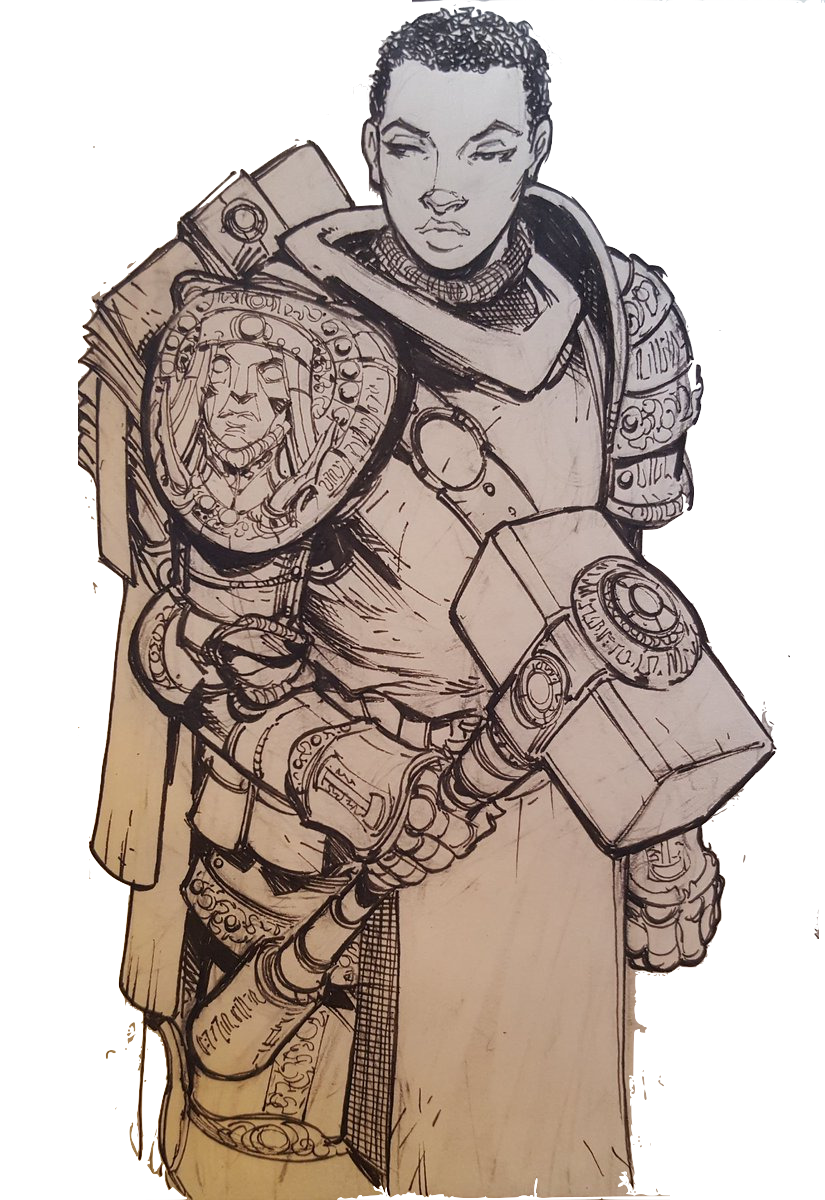
\includegraphics[width=\textwidth]{img/paladin-2.png}
{\scriptsize Art by Max Dunbar}
\end{Figure}
    
\end{multicols*}

    